\subsection{Contemporaneous Factorial and Evidence Controls}

\label{sec:eval:recovery_ablation}

After service recovery, we execute the frozen 840-request protocol as one new Gemma batch. All responses return and parse successfully without retries. Four generation settings cross preprocessing ($P$) and diagnostic context ($D$) on sixty controlled and sixty natural inputs (480 responses). Filtering ($G$) is scored with and without the same checks on each response. The other 360 responses compare six receipt-context settings on the sixty follow-up documents. These are reused evaluation documents; the original interrupted batch remains archived separately.

\begin{table}[t]

\centering

\caption{Factorial main effects in F1 percentage points, averaged over the other two switches. Each cohort has sixty paired documents. Intervals are marginal 95\% document-bootstrap intervals; $p_H$ uses Holm correction over six main effects.}

\label{tab:recovery_factorial}

\small

\begin{tabular}{llrrr}

\toprule

Input & Component & Change & 95\% interval & $p_H$ \\

\midrule

Controlled & Preprocessing & -0.028 & [-0.797, 0.778] & 1.000 \\

Controlled & Diagnosis & -0.651 & [-1.348, -0.056] & 0.164 \\

Controlled & Gate & +0.164 & [0.054, 0.301] & 0.156 \\

Natural & Preprocessing & +0.697 & [0.000, 1.905] & 1.000 \\

Natural & Diagnosis & -0.535 & [-2.376, 0.842] & 1.000 \\

Natural & Gate & +0.707 & [0.225, 1.316] & 0.086 \\

\bottomrule

\end{tabular}

\end{table}

None of the six main effects passes Holm correction (Table~\ref{tab:recovery_factorial}). Diagnostic context has a negative mean effect in both cohorts. Gate improves mean F1 by 0.164 points on controlled inputs and 0.707 points on natural inputs. Its full-check audit rejects 47 candidate occurrences across all cohorts: 17 have wrong heads and 30 lack source support; none exactly matches a reference triple. Interactions and per-check removals are released with the paired scores.

\begin{table}[t]

\centering

\caption{Receipt context controls with the same model, source and output budget. All rows include the same filter; sixty documents per row. Random context approximately matches index character length, not exact token count.}

\label{tab:recovery_index}

\small

\begin{tabular}{lrr}

\toprule

Context & Exact F1 & Normalized F1 \\

\midrule

Simple & 0.7917 & 0.8125 \\

Full index & 0.8351 & 0.8643 \\

Anchors only & 0.8351 & 0.8643 \\

Random index & 0.8167 & 0.8458 \\

Simple, no definitions & 0.8083 & 0.8292 \\

Full index, no definitions & 0.7470 & 0.7762 \\

\bottomrule

\end{tabular}

\end{table}

The full index leads Simple by 4.35 F1 points (95\% CI: 1.25 to 7.86), but the contrast has $p_H=0.065$ across the five prespecified comparisons. Full and anchors-only have identical mean F1; full minus random is 1.85 points (CI: $[-0.65,4.52]$, $p_H=0.696$). Removing field definitions from the full index lowers F1 by 8.81 points (CI: $[4.23,13.39]$, $p_H=0.006$), whereas definitions do not improve the simple arm in this batch. These controls support the combination of field definitions and indexed context, while leaving the added value of neighbouring lines and targeted rather than random context unresolved.

\begin{figure}[t]

\centering

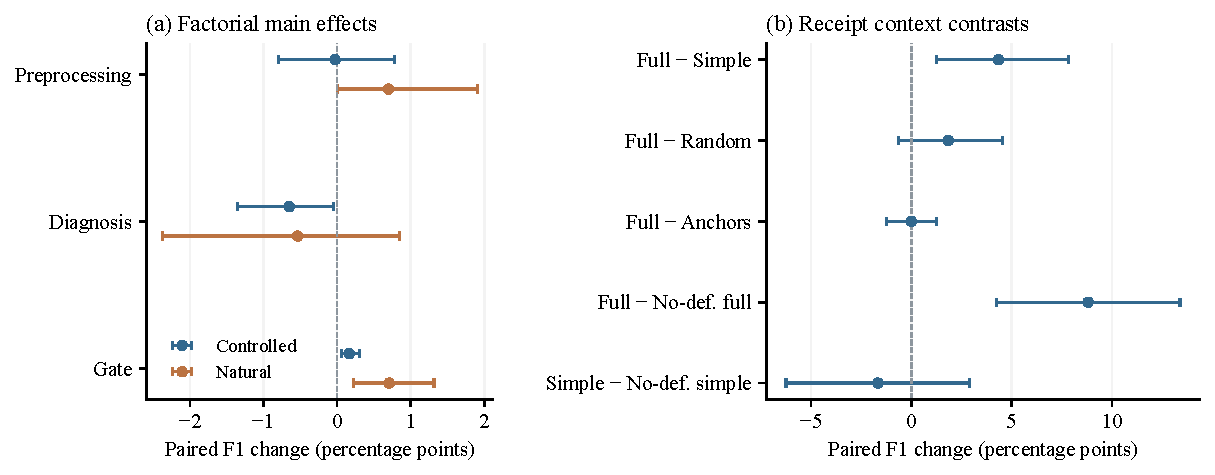
\includegraphics[width=0.98\textwidth]{figure/experiments/recovery_ablation.pdf}

\caption{Completed recovery controls. Points show paired mean F1 differences and bars show marginal 95\% document-bootstrap intervals. Main-effect and receipt-contrast families receive separate Holm corrections; intervals are not multiplicity-adjusted.}

\label{fig:recovery_ablation}

\end{figure}
